\section{Background}
\begin{figure}[t!]
  \centering
  % Requires \usepackage{graphicx}
  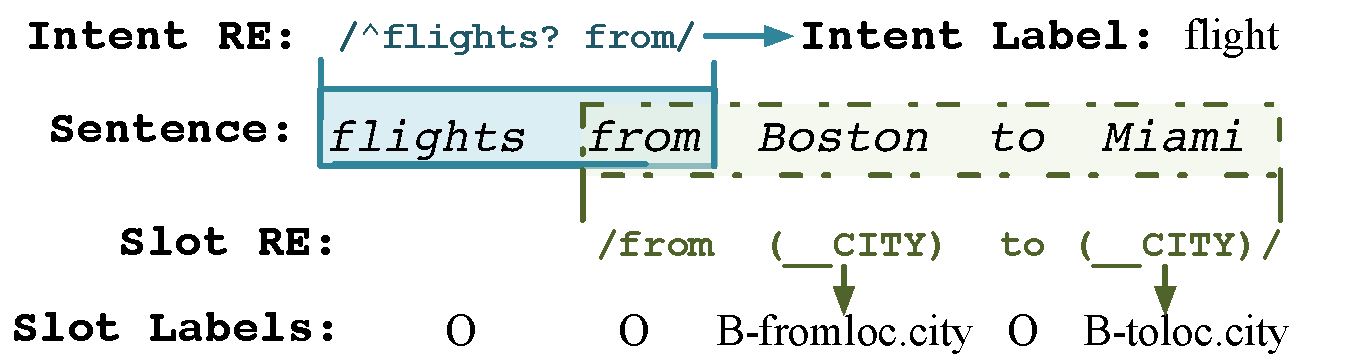
\includegraphics[width=0.49\textwidth]{figure/motivation.pdf}\\
  \caption{A sentence from the ATIS dataset. \REs can be used to detect the intent and label slots.}
  \label{atis_sample}
\end{figure}

\subsection{Problem Definition}
While our approach is generally applicable, to have concrete and measurable objectives, we apply it to two \SLU tasks: \emph{intent
detection} and \emph{slot filling}. The former is a sentence classification task where we learn a function to map an input sentence of $n$
words, $\textbf{x}=[x_{1}, ..., x_{n}]$, to a corresponding \textbf{\emph{intent label}}, $c$. The latter is a sequence labeling task for
which we learn a function to take in an input query sentence of $n$ words, $\textbf{x}=[x_{1}, ..., x_{n}]$, to produce a corresponding
labeling sequence, $\textbf{y}=[y_{1}, ..., y_{n}]$, where each element of the sequence, $y_i$, is the \textbf{\emph{slot label}} of the
corresponding word, $x_i$, in the input query.


%Intent detection is a typical sentence classification task.
%We need to learn a mapping function that maps an input sentence $\textbf{x}$, where $\textbf{x}=[x_{1}, ..., x_{n}]$ is the input sentence with $n$ words, to the corresponding intent $y$.
%% $f: \mathcal{X} \rightarrow \mathcal{Y}$
%% Given a set of training examples $\{(x_i, y_i): i=1,...,N\}$,
%
%On the other side, slot filling is often treated as a sequence labeling task.
%We need to learn a mapping function that maps an input query sentence $\textbf{x}$ to the corresponding label sequence $\textbf{y}$, where $\textbf{y}=[y_{1}, ..., y_{n}]$ is the slot labels of each word.
% Here we also have a set of training examples $\{(\textbf{x}_i, \textbf{y}_i): i=1,...,N\}$, where $\textbf{x}_i=[x_{i1}, ..., x_{in_i}]$ is the input sentence with $n_i$ words, and $\textbf{y}_i=[y_{i1}, ..., y_{in_i}]$ is the slot label of each word.

%For example, Figure\ref{atis_sample} shows a sample sentence in the ATIS dataset. Its intent is \emph{flight}, indicating the user wants
%flight-related information. We also need to identify the \emph{from\_city} and the \emph{to\_city} slots so that the we can return the
%correct information.

\cparagraph{Example} Fig.~\ref{atis_sample} gives an example sentence from the ATIS (Airline Travel Information Systems)
dataset~\cite{hemphill1990atis}. A successful intent detection would suggest the intent of the sentence is \emph{flight}, i.e., the query
is about flight-related information. Slot filling, on the other hand, would need to identify the slots \emph{fromloc.city} and
\emph{toloc.city} by labeling the sentence using e.g., the begin-inside-outside (\texttt{BIO}) scheme.




\subsection{The Use of Regular Expressions}
\label{re_desc}

In this work, a \RE defines a mapping from a text \emph{pattern} to several \textbf{\emph{\REtags}} which are related to or the same as the
\textbf{\emph{target labels}} (i.e., intent and slot labels). A search function takes in a \RE, applying it to a sentence, and returning
all texts that match the pattern. The search is designed to return every match on a sentence. If a matched pattern is found for a sentence,
a \REtag is assigned to either the entire sentence (for intent detection) or some phrases of the sentence (for slot filling).


\cparagraph{Intent Detection} 
% If a \REtag indicates an intent, it would be the same as an intent label.
In this work, the \REtags for intent detection is the same as the intent labels.
For example, applying the intent
\RE in Fig.~\ref{atis_sample} to the sentence given in the figure results in a \REtag that is equivalent to the intent label of
\emph{flight}.
\lb{I think "If a \REtag indicates an intent, it would be the same as an intent label." is a little confusing, since intent equals to intent label. So I changed it to the original version.}


% an \RE of \texttt{/\textasciicircum
% flights?\:from/} can be associated with an intention label \emph{flight}; and when applying this \RE to the sentence given in
% Figure~\ref{atis_sample} for intention detection, we get a \REtag of \emph{flight}.

\cparagraph{Slot Filling} We use two sets of \REs for slot filling. Given the group functionality of \RE, we can assign \REtags to our
interested \textbf{\emph{\RE groups}} (the text surrounded by parentheses). (1)~For the method in Sec.~\ref{interact_with_module}, since we
need to annotate clue words for certain slot labels, its \REtags are the same as the slot labels. For example, the slot \RE in
Fig.~\ref{atis_sample} will assign \emph{fromloc.city} to the first \RE group and \emph{toloc.city} to the second group. Here
\texttt{\_\_CITY} is a list of all the city names, which can be replaced with a string like \texttt{/Boston|Miami|LA/}. Note that, an
ordinary word list pattern can be written as strings like \texttt{/(\_\_CITY)/} in \RE. (2)~For the methods in Sec.~\ref{fusion_with_input}
and \ref{fusion_with_output}, the \REtag is different from the slot label. For example, the first and second \RE groups in the slot \RE of
Fig.~\ref{atis_sample} will all be tagged as \emph{city}, which is a simplified version of the slot label, and is related to three slot
labels: \emph{fromloc.city}, \emph{toloc.city}, \emph{stoploc.city}. The reason that we use different \REs here is to give an example that
\REs with output different from the target labels can also make improvements to \NN.

\z{The concept of \RE Groups is really confusing.}


\cparagraph{Generating \REs} For this work, the overhead in developing \REs mainly stemmed from two aspects. The first is the number of \RE
groups -- the more \RE groups we have, the higher precision we are likely to obtain, but a higher number of \RE groups also requires more
efforts to generate. The second is the number of expressions separated by the disjunction operator, `$|$', in a \RE. Having a
longer list of expressions can improve the coverage of the \RE, but writing the list also requires efforts. Later in this paper, we show
that it is worth to spend modest efforts in generating \REs, and our approach can adapt to \RE sets of different qualities to effectively
exploit the expressed knowledge.

% We use another set of \texttt{RE}s for the methods in Sec.~\ref{fusion_with_input} and \ref{fusion_with_output} because using simpler tags can significantly reduce the complexity of the \RE, and therefore making the generation of \RE much easier. For example, we need \texttt{/(from)\:(\_\_CITY)/} to identify \emph{fromloc.city}, but only \texttt{/(\_\_CITY)/} to identify \emph{city}.

%When writing \REs, since complicated \REs often lead to better performance but require more efforts to generate, \RE complexity is often an
%important trade-off that we need to make. Generally, two aspects affect the complexity most. First, \RE complexity increases with the
%number of \RE groups. This kind of complexity will lead to better precision but lower coverage. Second, \RE complexity also increases with
%the number of \emph{or}s (the symbol $|$) in a \RE group. Here a group can be considered as a set of phrases that express the same meaning.
%Therefore, this kind of complexity usually results in higher coverage and slightly lower precision.
% unless adding ambiguous phrases to the group

% Note that, while the outputs are the intent or slot themselves in the examples above, the \RE output can also be a tag related to, but not the same as, the label that we want to predict.
% We allow this variation because using tags different from the target labels can sometimes make it easier to write an \RE. For example, we need \texttt{/from\:(\_\_CITY)/} to identify \emph{fromloc.city}, but only \texttt{/(\_\_CITY)/} to identify \emph{city}. In this paper, the output of intent patterns is the same as the intent label, and the output of slot patterns used by the method in Section \ref{interact_with_module} is the same as the slot label. However, the slot \RE tag for methods in Section \ref{fusion_with_input} and \ref{fusion_with_output} is the entity part of the slot label (e.g., \emph{city} in \emph{fromloc.city}).
